\documentclass[tikz]{standalone}
\usetikzlibrary{decorations.pathreplacing} % Required for brackets

\begin{document}
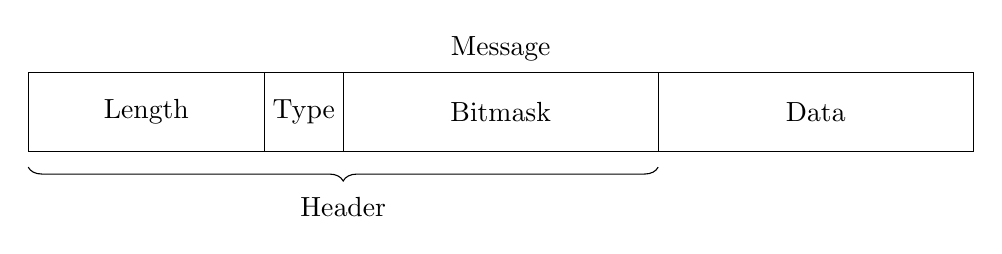
\begin{tikzpicture}
    % Drawing the message box
    \draw (0,0) rectangle (12,1);
    \node at (6,1.3) {Message};

    % Header components: Length, Type, Bitmask (4 bytes, 1 byte, 4 bytes)
    \draw (0,0) -- (0,1); % start
    \draw (3,0) -- (3,1); % length 4 bytes
    \draw (4,0) -- (4,1); % type 1 byte
    \draw (8,0) -- (8,1); % bitmask 4 bytes
    % Rest of the message follows

    % Labels for Length, Type, and Bitmask
    \node at (1.5,0.5) {Length};
    \node at (3.5,0.5) {Type};
    \node at (6,0.5) {Bitmask};

    % Label for Data
    \node at (10,0.5) {Data};

    % Bracket to indicate header
    \draw [decorate,decoration={brace,mirror,amplitude=5pt}] (0,-0.2) -- (8,-0.2);
    \node at (4,-0.7) {Header};
\end{tikzpicture}
\end{document}
